\PassOptionsToPackage{unicode=true}{hyperref} % options for packages loaded elsewhere
\PassOptionsToPackage{hyphens}{url}
%
\documentclass[
  ignorenonframetext,
]{beamer}
\usepackage{pgfpages}
\setbeamertemplate{caption}[numbered]
\setbeamertemplate{caption label separator}{: }
\setbeamercolor{caption name}{fg=normal text.fg}
\beamertemplatenavigationsymbolsempty
% Prevent slide breaks in the middle of a paragraph:
\widowpenalties 1 10000
\raggedbottom
\setbeamertemplate{part page}{
  \centering
  \begin{beamercolorbox}[sep=16pt,center]{part title}
    \usebeamerfont{part title}\insertpart\par
  \end{beamercolorbox}
}
\setbeamertemplate{section page}{
  \centering
  \begin{beamercolorbox}[sep=12pt,center]{part title}
    \usebeamerfont{section title}\insertsection\par
  \end{beamercolorbox}
}
\setbeamertemplate{subsection page}{
  \centering
  \begin{beamercolorbox}[sep=8pt,center]{part title}
    \usebeamerfont{subsection title}\insertsubsection\par
  \end{beamercolorbox}
}
\AtBeginPart{
  \frame{\partpage}
}
\AtBeginSection{
  \ifbibliography
  \else
    \frame{\sectionpage}
  \fi
}
\AtBeginSubsection{
  \frame{\subsectionpage}
}
\usepackage{lmodern}
\usepackage{amssymb,amsmath}
\usepackage{ifxetex,ifluatex}
\ifnum 0\ifxetex 1\fi\ifluatex 1\fi=0 % if pdftex
  \usepackage[T1]{fontenc}
  \usepackage[utf8]{inputenc}
  \usepackage{textcomp} % provides euro and other symbols
\else % if luatex or xelatex
  \usepackage{unicode-math}
  \defaultfontfeatures{Scale=MatchLowercase}
  \defaultfontfeatures[\rmfamily]{Ligatures=TeX,Scale=1}
\fi
% use upquote if available, for straight quotes in verbatim environments
\IfFileExists{upquote.sty}{\usepackage{upquote}}{}
\IfFileExists{microtype.sty}{% use microtype if available
  \usepackage[]{microtype}
  \UseMicrotypeSet[protrusion]{basicmath} % disable protrusion for tt fonts
}{}
\makeatletter
\@ifundefined{KOMAClassName}{% if non-KOMA class
  \IfFileExists{parskip.sty}{%
    \usepackage{parskip}
  }{% else
    \setlength{\parindent}{0pt}
    \setlength{\parskip}{6pt plus 2pt minus 1pt}}
}{% if KOMA class
  \KOMAoptions{parskip=half}}
\makeatother
\usepackage{xcolor}
\IfFileExists{xurl.sty}{\usepackage{xurl}}{} % add URL line breaks if available
\IfFileExists{bookmark.sty}{\usepackage{bookmark}}{\usepackage{hyperref}}
\hypersetup{
  pdftitle={Analyse BIP pro Kopf, Zufriedenheit Korrelationsanalyse},
  pdfborder={0 0 0},
  breaklinks=true}
\urlstyle{same}  % don't use monospace font for urls
\newif\ifbibliography
\usepackage{graphicx,grffile}
\makeatletter
\def\maxwidth{\ifdim\Gin@nat@width>\linewidth\linewidth\else\Gin@nat@width\fi}
\def\maxheight{\ifdim\Gin@nat@height>\textheight\textheight\else\Gin@nat@height\fi}
\makeatother
% Scale images if necessary, so that they will not overflow the page
% margins by default, and it is still possible to overwrite the defaults
% using explicit options in \includegraphics[width, height, ...]{}
\setkeys{Gin}{width=\maxwidth,height=\maxheight,keepaspectratio}
\setlength{\emergencystretch}{3em}  % prevent overfull lines
\providecommand{\tightlist}{%
  \setlength{\itemsep}{0pt}\setlength{\parskip}{0pt}}
\setcounter{secnumdepth}{-2}

% set default figure placement to htbp
\makeatletter
\def\fps@figure{htbp}
\makeatother


\title{Analyse BIP pro Kopf, Zufriedenheit Korrelationsanalyse}
\date{}

\begin{document}
\frame{\titlepage}

\begin{frame}[fragile]

\begin{verbatim}
## 
## Attaching package: 'dplyr'
\end{verbatim}

\begin{verbatim}
## The following objects are masked from 'package:stats':
## 
##     filter, lag
\end{verbatim}

\begin{verbatim}
## The following objects are masked from 'package:base':
## 
##     intersect, setdiff, setequal, union
\end{verbatim}

\begin{block}{Top 10 Economies by GDP - 2007}

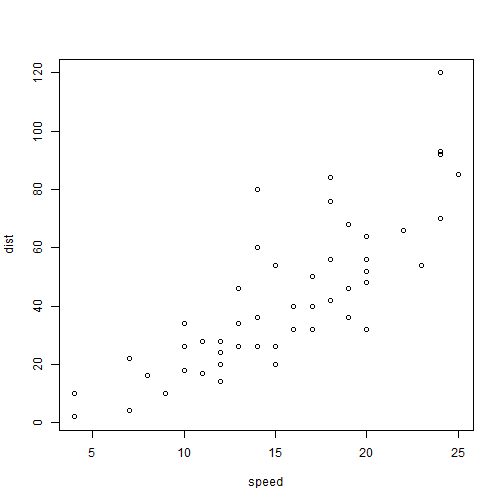
\includegraphics{Slidy_files/figure-beamer/unnamed-chunk-2-1.pdf}

\end{block}

\begin{block}{Entwicklung der Lebenserwartung Schweiz und USA 1952 -
2007}

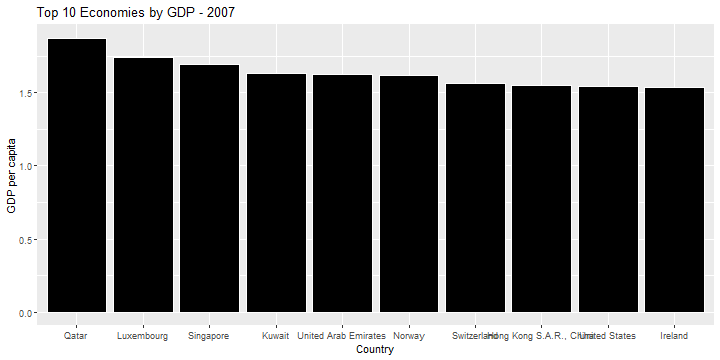
\includegraphics{Slidy_files/figure-beamer/unnamed-chunk-3-1.pdf}

\end{block}

\end{frame}

\begin{frame}{Korrelation Lebenserwartung und BIP pro Kopf weltweit
zwischen 1952 und 2007}
\protect\hypertarget{korrelation-lebenserwartung-und-bip-pro-kopf-weltweit-zwischen-1952-und-2007}{}

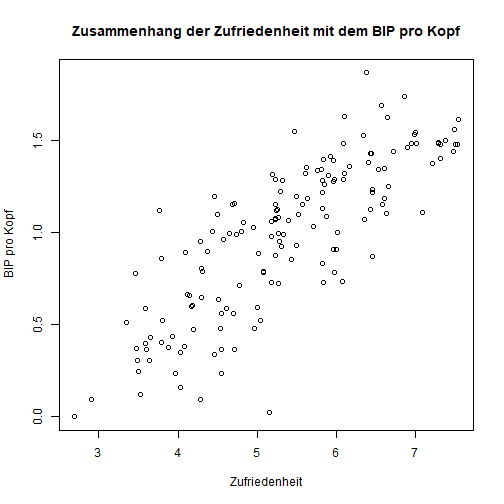
\includegraphics{Slidy_files/figure-beamer/unnamed-chunk-4-1.pdf}

\end{frame}

\begin{frame}{Bevölkerungsentwicklung Schweiz 1952 - 2007}
\protect\hypertarget{bevolkerungsentwicklung-schweiz-1952---2007}{}

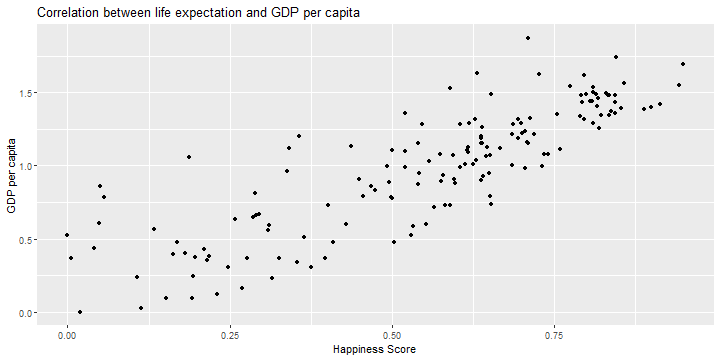
\includegraphics{Slidy_files/figure-beamer/unnamed-chunk-5-1.pdf}

\end{frame}

\begin{frame}{Korrelation der Zufriedenheit mit dem BIP pro Kopf}
\protect\hypertarget{korrelation-der-zufriedenheit-mit-dem-bip-pro-kopf}{}

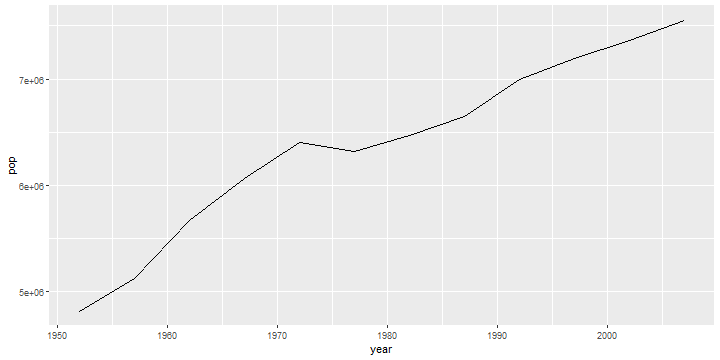
\includegraphics{Slidy_files/figure-beamer/unnamed-chunk-6-1.pdf}

\end{frame}

\begin{frame}{Korrelation zwischen Zufriedenheit und Freiheit}
\protect\hypertarget{korrelation-zwischen-zufriedenheit-und-freiheit}{}

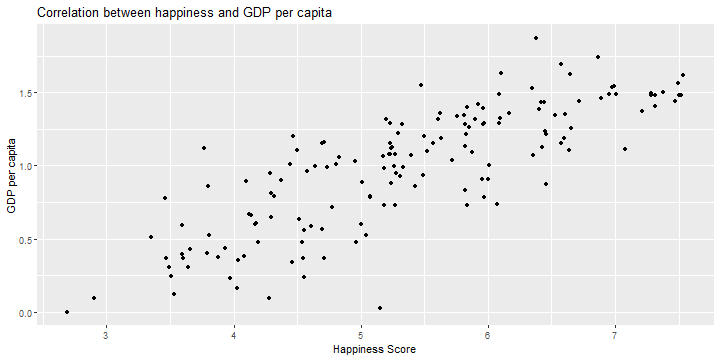
\includegraphics{Slidy_files/figure-beamer/unnamed-chunk-7-1.pdf}

\end{frame}

\end{document}
